\listfiles
\documentclass[twoside,12pt]{article}
\newcommand{\dataset}{{\cal D}}
\newcommand{\fracpartial}[2]{\frac{\partial #1}{\partial  #2}}
\usepackage{hyperref}
\usepackage{enumerate}
\usepackage[top=2in, bottom=1.5in, left=0.85in, right=0.5in]{geometry}
\usepackage[hyphenbreaks]{breakurl}
%\usepackage[pdfstartview=FitH,pdfstartpage=13,pdfpagemode=UseNone]{hyperref}
\usepackage{amsfonts}
\usepackage{graphicx} 
\usepackage[linesnumbered,ruled]{algorithm2e}
\usepackage{float}
\usepackage{amssymb,amsmath}
\usepackage{mdwlist }
\usepackage{color}
\usepackage{multirow}
\usepackage{listings}
\usepackage{float}
\usepackage{setspace}
\usepackage[english]{babel}

\definecolor{darkblue}{rgb}{0.0,0.0,0.5}
\newtheorem{Dfn}{Definition}
\hypersetup{colorlinks,breaklinks,
            linkcolor=darkblue,urlcolor=darkblue,
            anchorcolor=darkblue,citecolor=darkblue}
\newcommand{\sign}{\text{sign}}
\newcommand{\argmin}{\arg\!\max}
\begin{document}

\title{Parameter estimation for text analysis\\  Learning Algorithms, Project 3}
\author{Mohsen Malmir, Erfan Sayyari}
\maketitle
\section{Abstract}


\section{Introduction}



\section{Design and Analysis of Algorithm}

\subsection{The bag-of-words representation}
A document is a collection of words and the structure that puts these words together. If we only look at words, we find some words that are not correlated with any topic. These are words that can be found in any document with any topic. Examples of these words are pronouns (you, he, it) connectives (and, because, however), prepositions (to, of, before), auxiliaries (have, been, can), and generic nouns (amount, part, nothing). For the purpose of topic selection, we discard these words from documents as clearly they don't help in picking the right topic. Then we take the union of all words in corpus and call it \emph{dictionary}.

In order to determine a topic for a document, we have to represent  documents using a set of features. We adapt a representation called \emph{bag of words}, in which each document is represented as a histogram over the dictionary. Let $V$ be the total number of words in the dictionary, then each document is represented as a $V$-dimensional vector $x$, where $x[i]$ is the number of times the $i$th word appeared in the document. We can calculate the length of the document as $n=\sum_{m}x_j.$

\subsection{Latent Dirichlet Allocation Model}
To learn the topic distribution for documents, we use the model shown in figure \ref{figGM}. This is a model of $M$ documents, each with length $n_m$. Each word in a document comes from a \emph{topic} $z$. A topic is modeled as a multinomial distribution over the dictionary, with $\phi_k$ as vector. Note that $\phi_k[i]$ denotes the probability that topic $k$ gives to the $i$th word in the dictionary. A document is modeled as a multinomial distribution over topics, with $\theta$ representing the parameters. Again, $\theta_m[i]$ represents the probability of having topic $i$ in the $m$th document. Finally, we put Dirichlet priors over document and topic distributions. The prior over documents is represented by the node $\alpha$, and denotes the prior belief in the distribution of topics in different documents. Also, the prior over topics is represented by node $\beta$, and denotes the prior belief of distribution of words in topics.

\begin{figure}[h!]
\centering
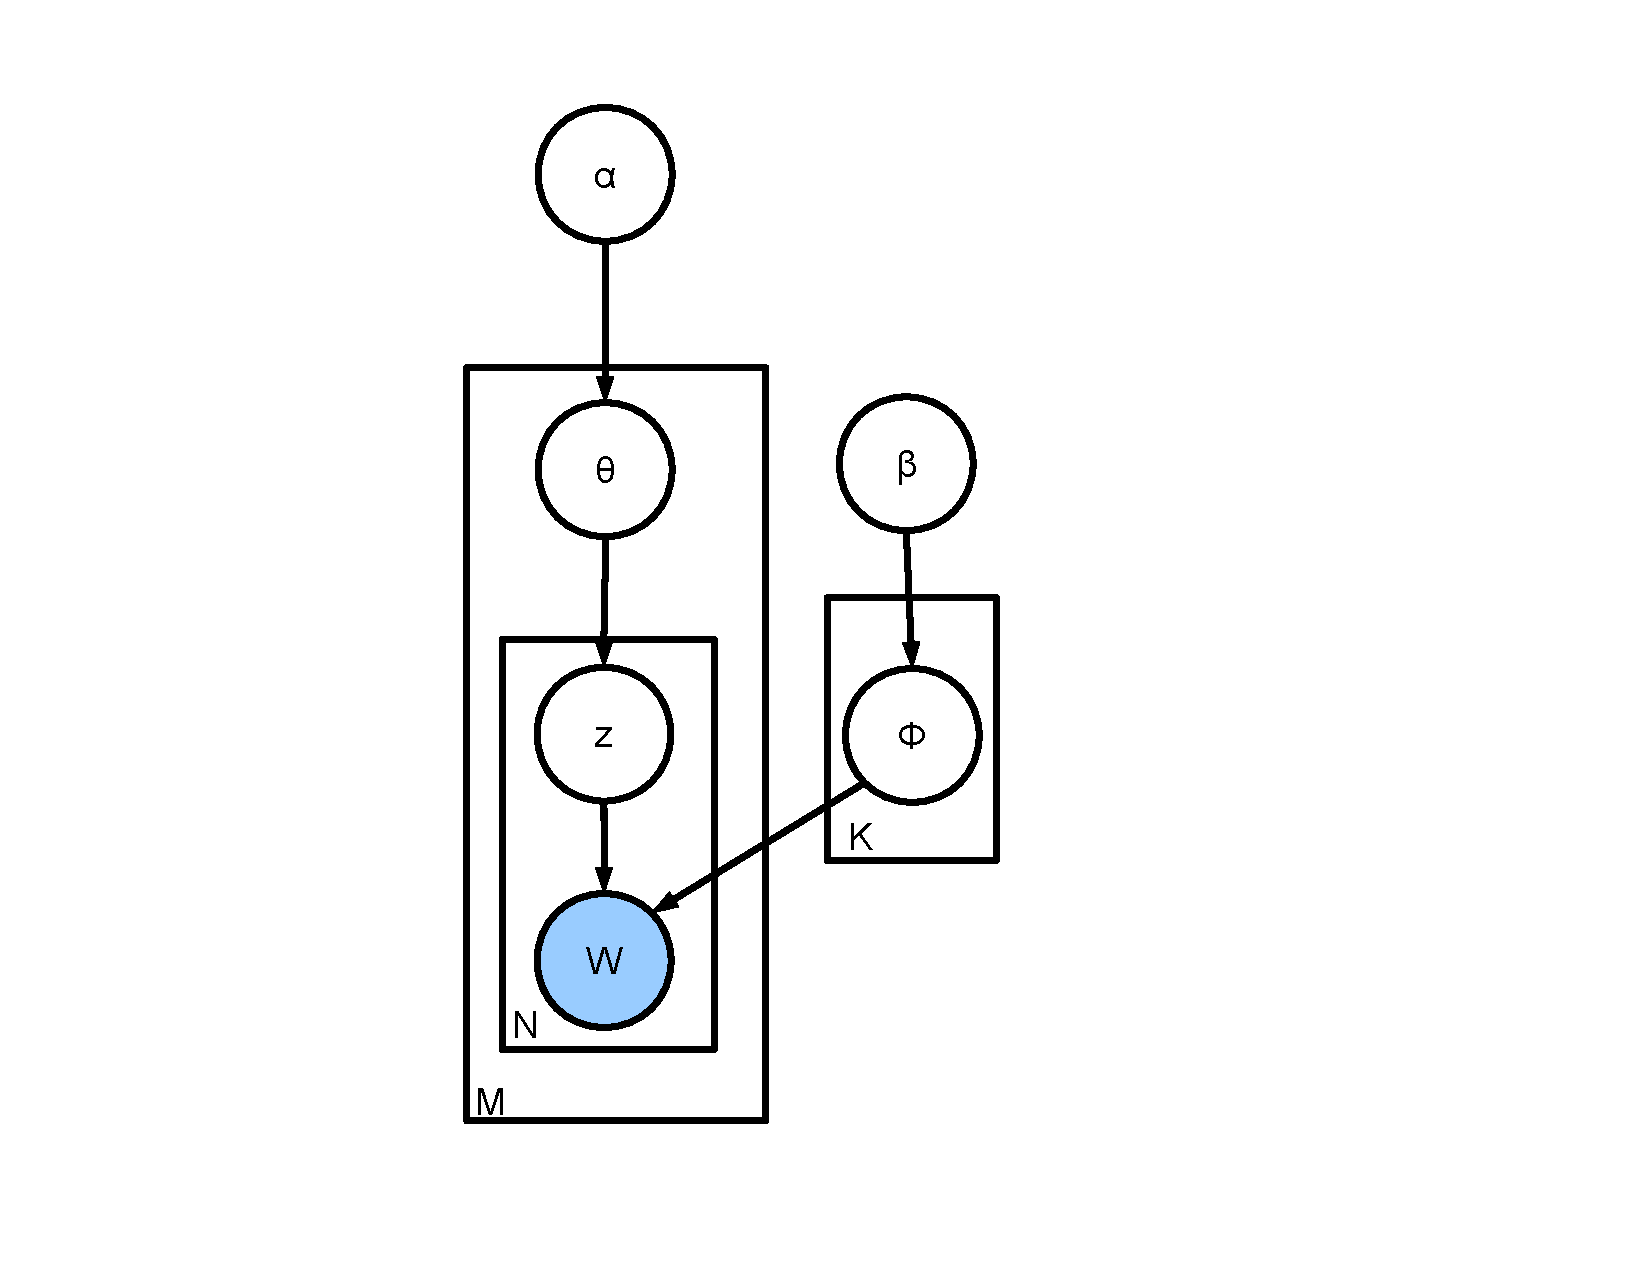
\includegraphics[width=.3\textwidth]{./figs/gm.pdf}
\caption{Plate notation of the LDA graphical model. The shaded node $w$ is observed. }
\label{figGM}
\end{figure}

The probability distribution represented by the graphical model in figure \ref{figGM} is,

\begin{align}
P(\alpha,\Theta,&Z,\beta,\Phi,W)  \\  &=P(\alpha) P(\beta) P(\Theta | \alpha) P(\Phi|\beta) P(Z|\Theta) P(W|Z,\Phi) \\ &= Dir(\alpha) Dir(\beta) \prod_{m=1}^M \text{Multi}(\theta_m | \alpha) \prod_{k=1}^K \text{Multi}(\phi_k | \beta) \prod_{t=1}^T \text{Multi}(w_t | \phi_{z_t})
\end{align}
 
 In the formula above, $\Phi = \{\phi_k, k=1,\ldots,K\}$ and $\Theta=\{\theta_m, m=1,\ldots,M\}$, $Dir$ represents Dirichlet and Multi represents the multinomial distributions. Also, $W = \{w_t, t=1,\ldots,T\}$ represents the entire set of words in the corpus. Note that the prior over topics and documents is chosen to be conjugate,
 
\begin{align}
\gamma \sim Dir(\alpha) \Rightarrow P(\gamma | \alpha) = \frac{\Gamma(\sum_{i=1}^M \alpha_i)}{\prod_{i=1}^M \Gamma(\alpha_i)} \prod_{i=1}^M \gamma_i^{\alpha_i -1} 
\end{align}
where
\begin{align}
\Gamma(t) = \int_0^\infty x^{t-1} e^{-x} dx
\end{align}
is the extension of Factorial function to continuous variables.
\subsection{ LDA Generative process}
To better understand the LDA model, we can look at how documents are generated in this model. First, $\phi_k, k=1,\ldots,K$ are randomly drawn from $Dir(\beta)$. Then For document $m, m=1,\ldots,M$, $\theta_m$ is sampled from $Dir(\alpha)$. Then $n_m$ topics are randomly drawn from Multi$(\theta_m)$. Given $z_t$, the $t$th word is selected from $\phi_{z_t}$.


\subsection{Inference}
Inference includes determining $\theta_m, \phi_k$ for $m=1,\ldots,M,\;\; k=1,\ldots,K$.


\subsection{Training via Gibbs sampling}
The training data are the words in all documents, and the prior distribution parameters $\alpha$, $\beta$, the number of topics $K$, number of documents $M$, length of each document $N_m$, and the length of vocabulary $V$ are assumed to be fixed and known.

Moreover, we suppose that we know the $z$ value for every word except for word number $i$. We want to draw the value for $z_i$ based on the probability distribution of topics and words. We use the notation $\overline{w'}$ to mean $\bar{w}$ with word number $i$ removed, so $\bar{w}=\{w_i,\overline{w'}\}$. Similarly, we write $\bar{z}=\{z_i,\overline{z'}\}$, and we need to compute the probability of $z_i$ given $\overline{z'},\bar{w}$:
\begin{equation}
p(z_i|\overline{z'},\bar{w})=\frac{p(\bar{z},\bar{w})}{\overline{z'},\bar{w}}=\frac{p(\bar{w}|\bar{z})p(\bar{z})}{p(w_i|\overline{z'})p(\overline{w'}|\overline{z'})p(\overline{z'})}
\end{equation}
for $z_i=1$ to $z_i=K$. After simplifications we could write this probability as:
\begin{equation}
p(z_i=j|\overline{z'},\bar{w})\propto \frac{q'_{jw_j}+\beta_{w_j}}{\sum_t q'_{jt}+\beta_t}\frac{n'_{mj}+\alpha_j}{\sum_k n'_{mk}+\alpha_k}.
\end{equation}
where $q_{kt}$ is the number of times that word $t$ occurs with topic $k$ in the whole corpus, and $q'_{jt}$ is equal to $q_{jt}$ with one subtracted from the count for word $t$ with topic $j$. $\overline{n'}_{m}$ is $\overline{n}_m$ with one subtracted from the count for topic $z_i$, and $\overline{n}_m$ is the vector of topic counts $\langle n_{m1},\ldots,n_{mK} \rangle$ for document number $m$.

\section{Design of Experiments}

\subsection{Dataset Selection}
The experiments on the model described above was done using two datasets: classic400 and dailyKOS. Table \ref{tableDatasetStats} display the number of documents, words and total number of words in these datasets. Classic400 is a small dataset, and the fact that it is accompanied by true labels makes it appealing for experiments. DailyKOS on the other hand is a larger dataset, and though it doesn't have the true labels, its large number of documents and total number of words makes it a good test to the performance of the proposed model. 


\begin{table}
\vspace{-2cm}
\center
\begin{tabular}{|c|c|c|}
\hline
 & \textbf{Classic400} & \textbf{DailyKOS} \\
 \hline
\textbf{ number of Documents} & 400 & 3430 \\
\textbf{ Dictionary Size} & 6205 & 6906 \\
\textbf{ Total Number of Words} & 31516 & 467714\\
 \hline
\end{tabular}
\caption{Statistics of classic400 and DailyKOS datasets.}
\label{tableDatasetStats}
\end{table}


\subsection{Hyperparameters Selection}
There are two sets of hyper parameters in our model: $\alpha$ which is the parameters of the Dircihlet prior over documents and $\beta$ which is the vector of parameters for Dirichlet prior over topics. One way to select these parameters is to use expert knowledge in determining these parameters. In this case, the expert can give an estimate of the distribution of topics inside documents or distribution of words for different topics. Despite enriching the model, this method seems infeasible for us since we have no source of expertise in this area. Another way is to use an uninformative uniform prior, which acts as psuedo-counts to prevent technical difficulties.\\
Here, we adapt the same parameter values as \cite{fastlda}: $\alpha \in \{0.01,0.1\}$ and $\beta\in\{2/k,0.2/k\}$. These value make sense since they prefer sparse distributions for $\theta$ and $\phi$. Usually documents contain a few topics, therefore a document is usually a sparse distribution over topics. Also when the dictionary size is large, it makes sense to have a topic that is sparse, i.e. it gives higher probability to a few words. Besides the sparsity, there is no other information we are incorporating in our priors. 

\section{Results}


\subsection{Classic400}
For classic400 dataset, we 


\begin{table}[!]
\begin{center}
\begin{tabular}{| c | p{12cm} |}
\hline
\textbf{Topic}& \textbf{Top 20 Words}  \\ \hline
\textbf{1}&boundary,layer,wing,mach,supersonic,wings,ratio,velocity,schlock, effects,surface,plate,solution,jet,lift,numbers,high,edges,speeds,head\\ \hline
\textbf{2}&system,scientific,retrieval,research,language,science,journals, methods,systems,subject,library,request,classification,data,problems, field,development,considered,general,structure\\
 \hline
\textbf{3}&ventricular,fatty,left,nickel,cases,acids,aortic,blood,normal,glucose, spetal,acid,pulmonary,defect, visual,time,clinical,free,ffa\\
 \hline
 
\end{tabular}
\caption{}
\label{table:2}
\end{center}
\end{table}


\subsection{DailyKOS}

\section{Discussion}


\begin{thebibliography}{9}
\bibitem{fastlda}
Porteous, Ian, et al. "Fast collapsed gibbs sampling for latent dirichlet allocation." Proceedings of the 14th ACM SIGKDD international conference on Knowledge discovery and data mining. ACM, 2008.

\end{thebibliography}




\end{document}
